\documentclass{article}

\title{Repairing a Lenovo ThinkPad Series 3 Mini Dock Plus (4337) with Hot Glue}
\author{LAK132}

\begin{document}

\maketitle

A ThinkPad dock I bought for my X220 arrived in less than stellar condition.
For whatever reason, when I placed the X220 on top of it,
it would not latch on.
I decided to open it up, and discovered that part of the mechanism that allows
the spring loaded top plate to lower and also reset the latches after the
laptop has been released, was damaged:

\includegraphics[width=19em]{images/IMG_6034.JPG}
\includegraphics[width=19em]{images/IMG_6036.JPG}
\includegraphics[width=19em]{images/IMG_6037.JPG}

As far as I can tell, this part was probably never going to last long,
given how much force it was under and the fact it was made from soft plastic.
At this point I had 2 options, I either repair the broken part,
or try and bypass the mechanism all together.
My initial attempt to repair the part didn't end well,
the super glue I used didn't want to stick to the plastic.
However, it turns out that this mechanism can be safely removed all together,
so long as the latch release mechanism is jammed:

\begin{figure}
	\caption{}
	\includegraphics[width=55em]{images/IMG_6041.JPG}
\end{figure}

\begin{figure}
	\caption{Top plate with latch reset/lowering mechanism removed}
	\includegraphics[width=55em]{images/IMG_6044.JPG}
\end{figure}

\begin{figure}
	\caption{Latch reset mechanism jammed with hot glue}
	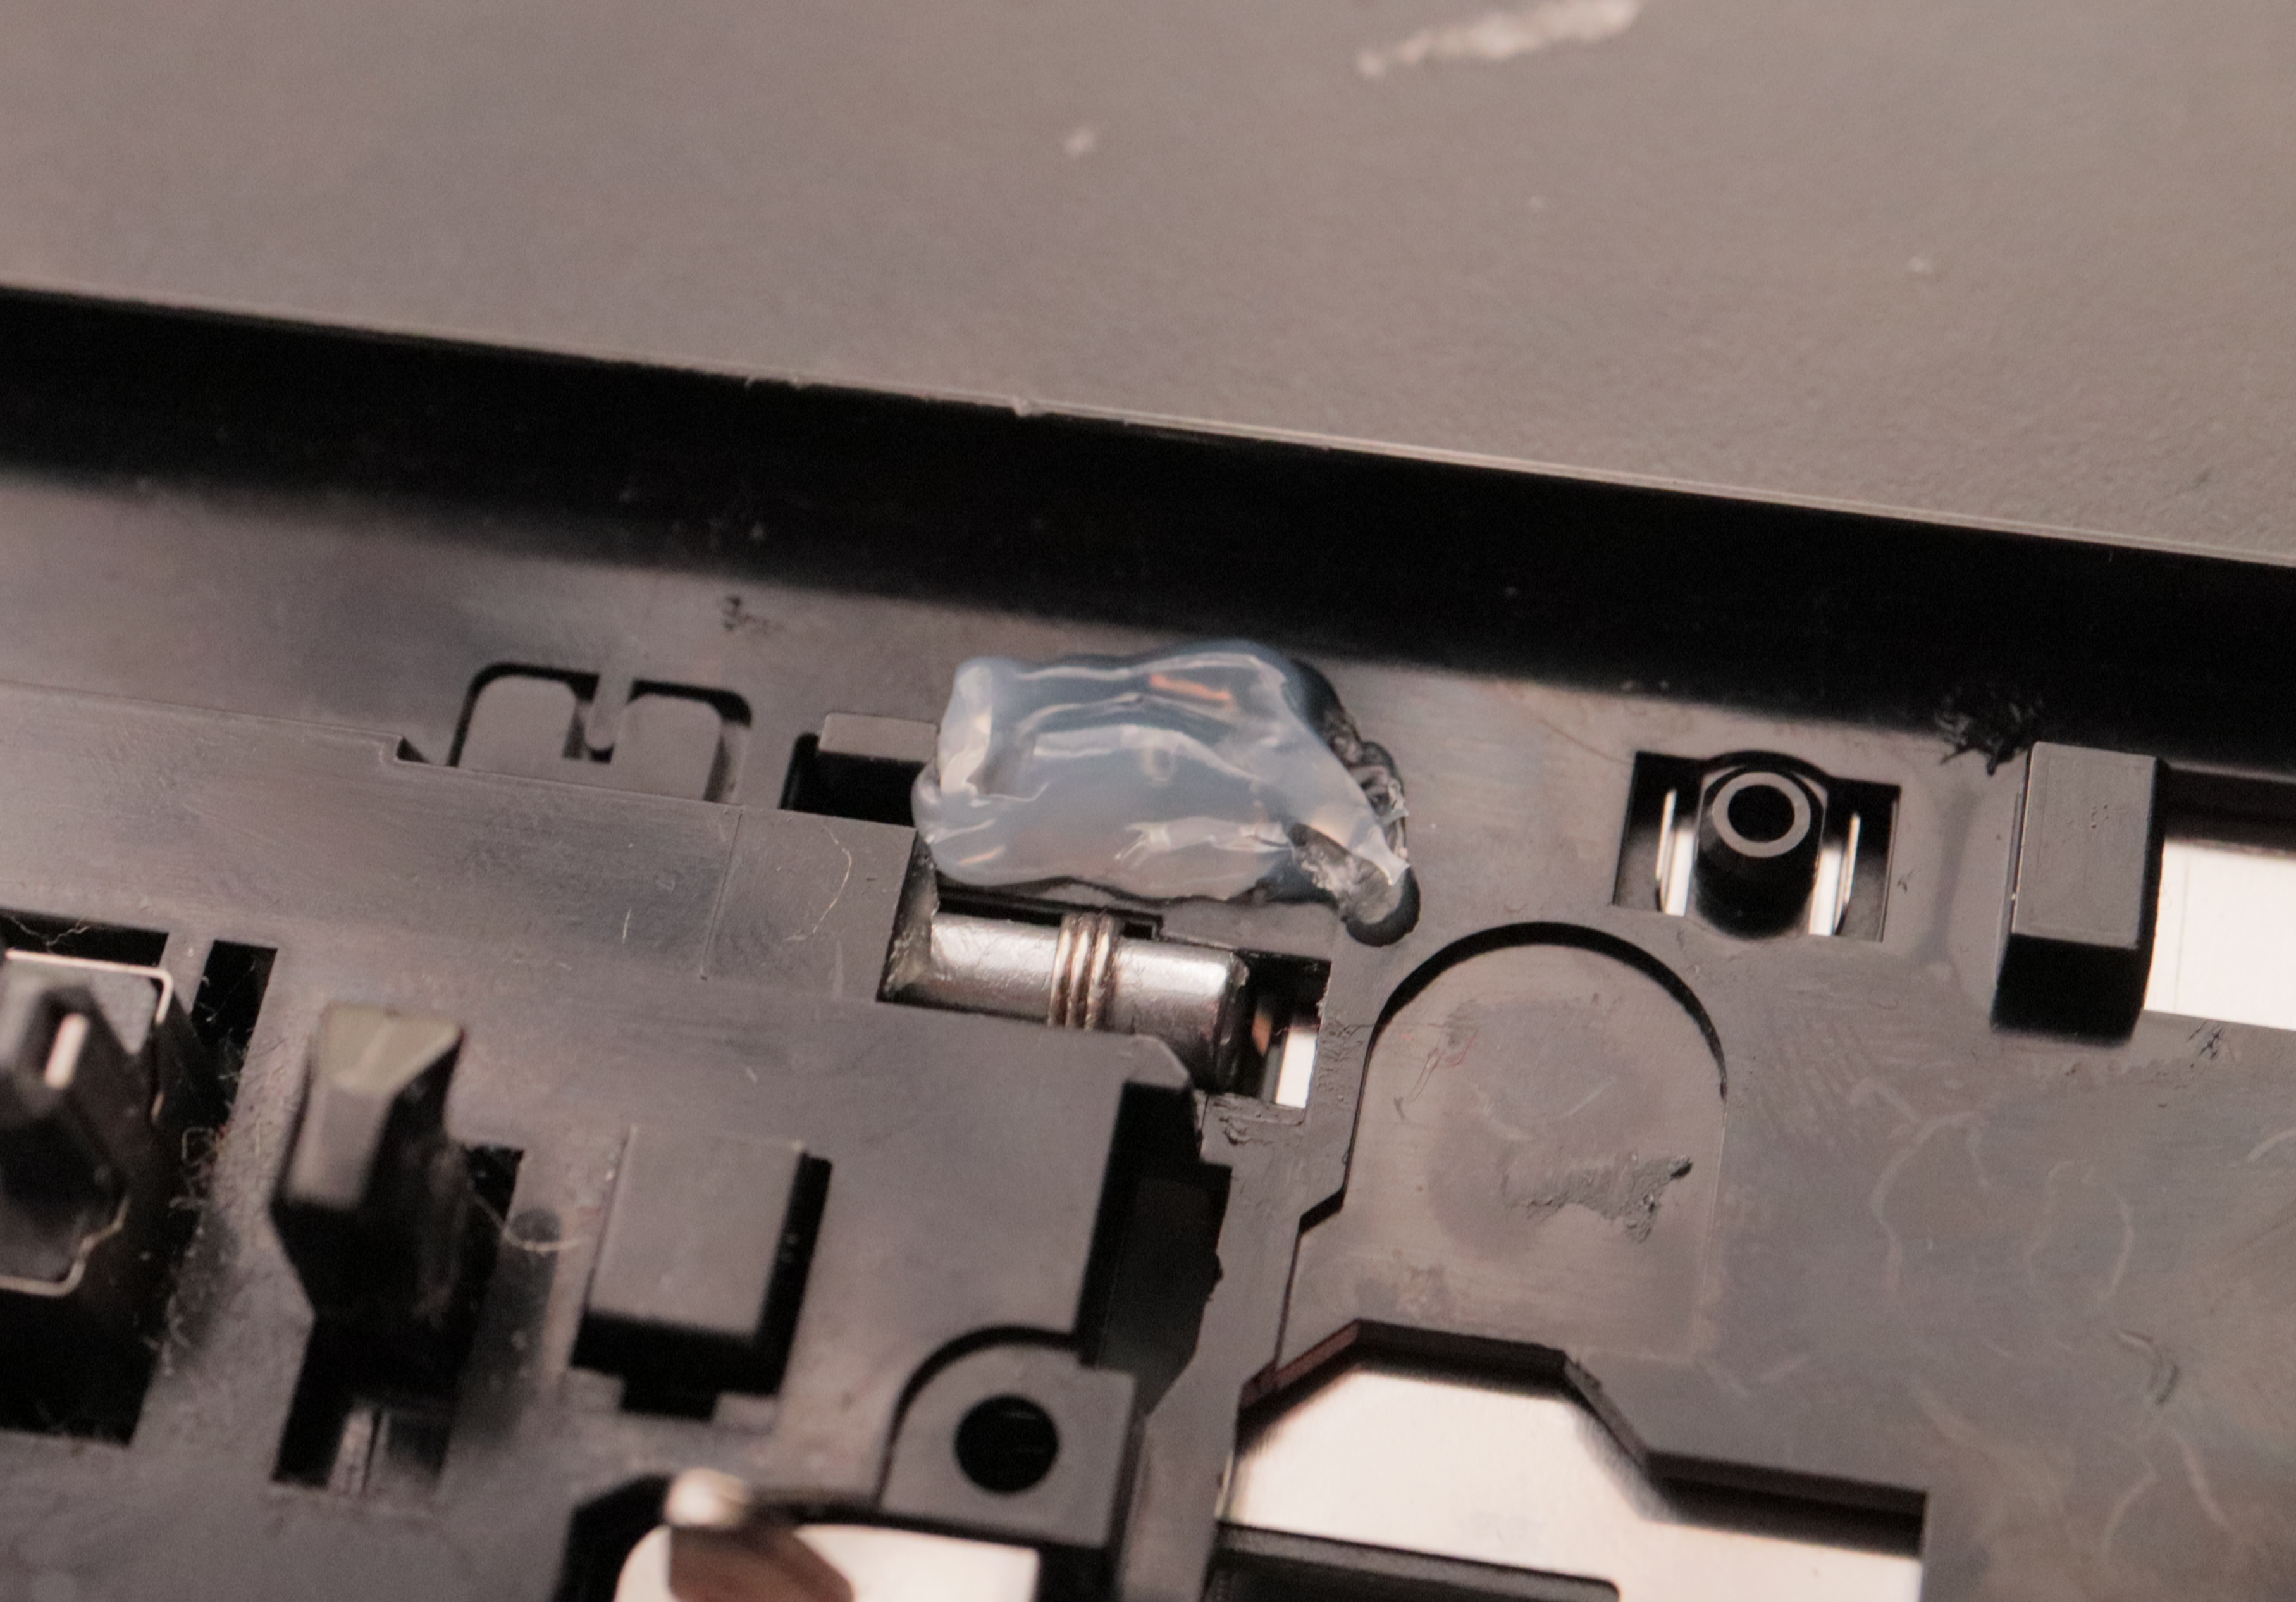
\includegraphics[width=55em]{images/IMG_6047.JPG}
\end{figure}

With it reassembled with the top plate mechanism removed and the latch reset
mechanism jammed with hot glue, the top plate will now lower all the way:

\begin{figure}
	\caption{}
	\includegraphics[width=55em]{images/IMG_6049.JPG}
\end{figure}

And the X220 will happily latch on!

\end{document}
